\chapter{Introduction}
\label{cha:introduction}

\section{Overview and aims}
%original work
The stratosphere is the second layer of the atmosphere above the Earth's
surface, bounded by the tropopause below and the stratopause above. The height
of the tropopause varies from about 15~km in altitude in the tropics to 7~km at
high latitudes, while the stratopause lies at approximately 50~km. The defining
feature of the stratosphere is a temperature gradient increasing with height (in
contrast to the troposphere below), caused by the presence of ozone which
absorbs ultraviolet radiation\footnote{For this reason, the region of the
  stratosphere with the highest ozone concentrations is often called the ``ozone
  layer''.}. This temperature gradient makes the stratosphere stable against
vertical convection and results in very different dynamical behaviour to the
troposphere.

Traditionally, the stratosphere was thought to respond passively to tropospheric
forcing from below. However, modelling and observational evidence accrued over
approximately the last two decades has suggested that the variability of the
winter polar stratosphere can cause consistent circulation anomalies at the
Earth's surface. Stratosphere-troposphere coupling has been found to be
particularly strong following the rapid breakdown of the 

Despite these advances, many questions remain as to the
stratosphere's influence on the troposphere. Firstly, it is not understood why
some types of stratospheric event appear to have a larger impact on the
stratosphere than others


\subsection{Relation to published work}
Chapter \ref{cha:moments} is largely based on a paper written by myself, Daniel
Mitchell and Lesley Gray in \emph{Geophysical Research Letters}
\citep{Seviour2013}, although the analysis has been significantly extended and
re-written. The results in Chapter \ref{cha:seas} on the Southern Hemisphere are
based on a paper written by myself, Steven Hardiman, Lesley Gray, Neal Butchart,
Craig MacLachlan, and Adam Scaife in \emph{Journal of Climate}
\citep{Seviour2014}. 

In both of these papers, all the writing is my own and I carried out all the
analysis and produced the figures. However, I am of course very grateful for the
constructive comments of my coauthors in the preparation of these papers as well
as my reviewers; Harry Hendon (from the Centre for Australian Weather and
Climate Research), and three of whom are anonymous.



\section{Dynamics of the polar stratosphere}

\subsection{Zonal mean flow}

Each winter the polar regions descend into a polar night and the stratosphere
cools by infrared radiation to space. This sets up a strong meridional
temperature gradient which increases the vertical zonal wind shear in accordance
with the thermal wind balance relation
\begin{equation}
\frac{\partial u_g}{\partial z} = -\frac{R}{fH}\frac{\partial T}{\partial y} \,, 
\end{equation} 
where $u_g$ is the geostrophic zonal velocity, $u_g = -Z_y/f$, $Z$ is
geopotential height, $f$ is the Coriolis parameter, $f=2\Omega\sin\phi$, and $R$
is the specific gas constant. Here, a beta-plane geometry is used such that
$f=f_0+\beta y$, where $f_0=f(\phi_0)$ and $\beta = 2\Omega a^{-1}\cos\phi_0$,
$a$ is the Earth's radius and $\phi_{0}$ is a reference latitude. $H$ is the
scale height given by $H = RT_s/g$, where $T_s$ is a reference temperature and
$g$ is the acceleration due to gravity. This equation relies on hydrostatic and
geostrophic approximations but is approximately satisfied on seasonal
timescales. Hence, the meridional temperature gradient decreasing from equator
to pole results in a region of westerly winds surrounding the pole; this is
known as the stratospheric polar vortex.

\begin{figure}
 \centering
 \noindent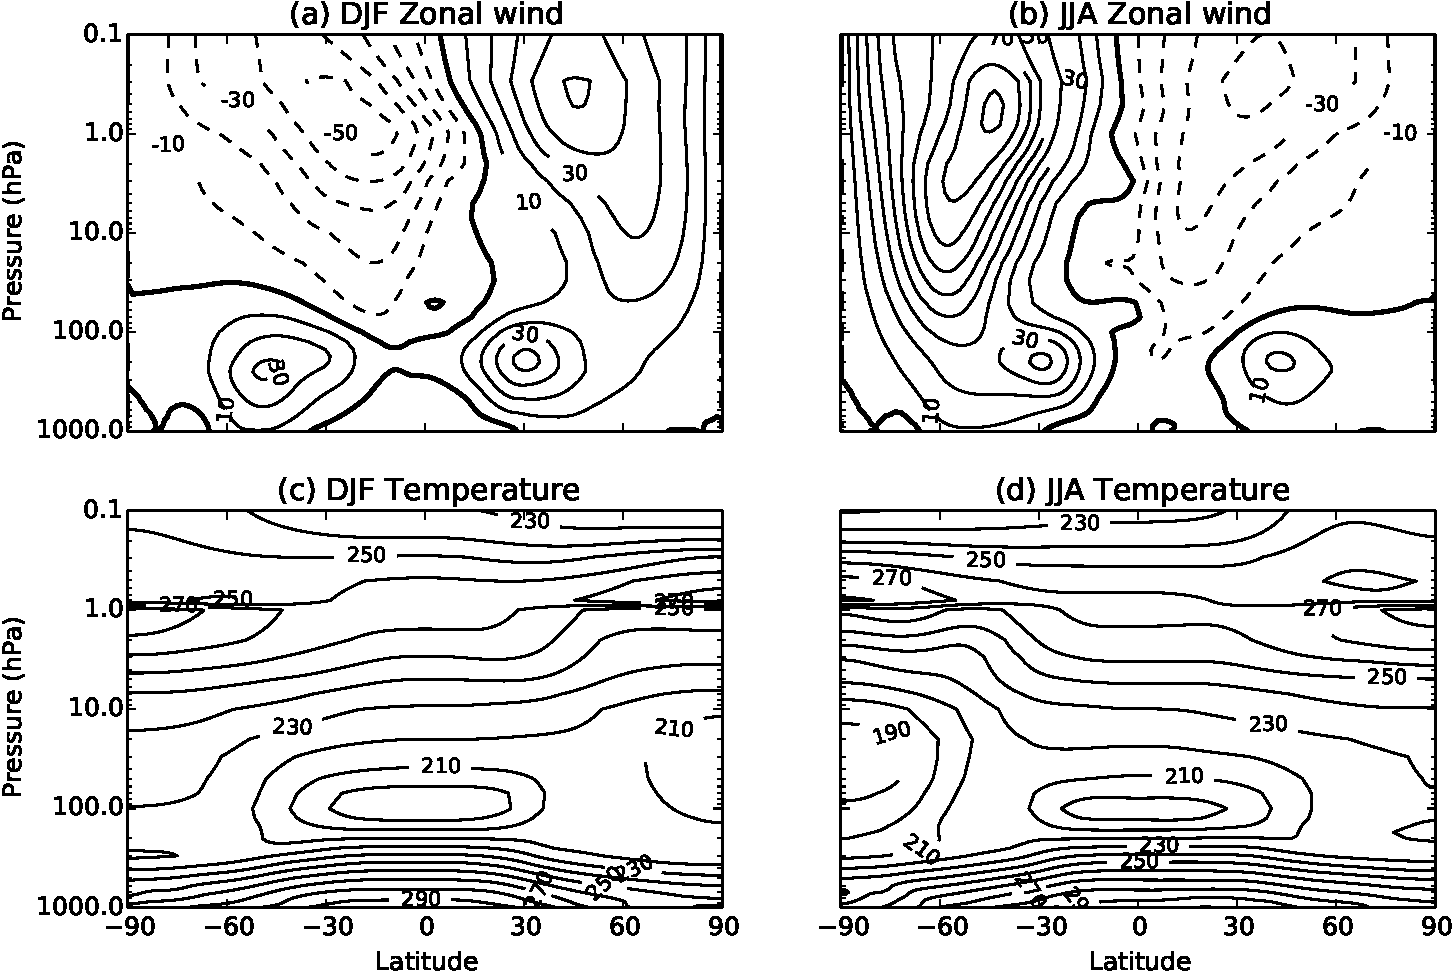
\includegraphics[width=\textwidth]{figures/chapter-intro/zmzw_zmT_clim.pdf}
 \caption[Zonal-mean zonal wind and temperature climatology.]{December-Janurary
   (DJF) (a,c) and July-August (JJA) (b,d) averages of zonal-mean zonal wind
   ($\mathrm{m~s^{-1}}$) (a,b) and temperature (K) (c,d). Data is from the
   ERA-Interim reanalysis (1979-2010).}
 \label{fig:zmzw_zmT_clim}
\end{figure}

Figure \ref{fig:zmzw_zmT_clim} shows zonal-mean zonal wind and temperature
averaged over the boreal winter (December-February; DJF) and austral winter
(July-August; JJA) using data from 1979-2010 from the ERA-Interim reanalysis
(details in Section \ref{sec:reanalysis-data}). In both cases the westerly
vortex in the winter hemisphere can be seen along with a local minimum in
temperature at the winter pole in the lower stratosphere. Weaker easterly winds
are present in the summer hemisphere. The maximum strength of the polar vortex
occurs at midlatitudes between 0.1-1~hPa in the mesosphere, and is stronger in
the Southern Hemisphere (SH) with a maximum of $90~\mathrm{ms^{-1}}$ than the
Northern Hemisphere (NH) with a maximum of $50~\mathrm{ms^{-1}}$. The winter
polar stratosphere is also approximately 20~K colder in th SH than the NH. 

\begin{figure}
 \centering
 \noindent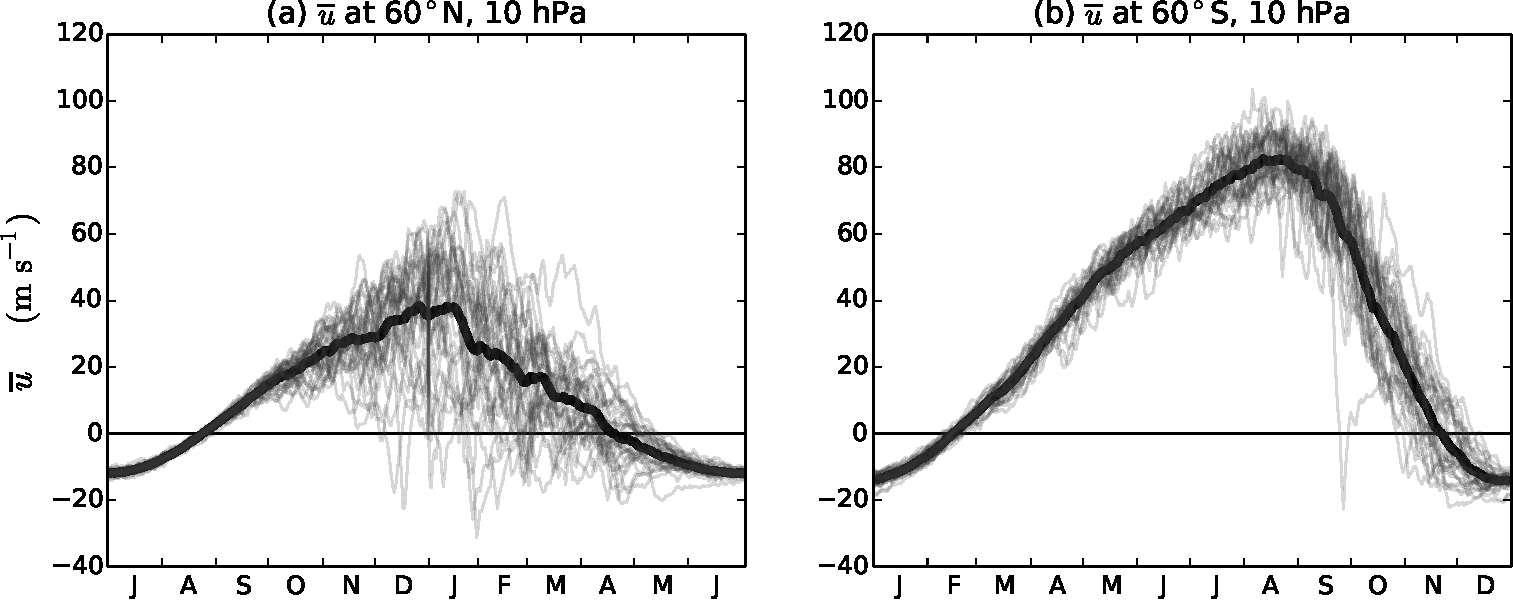
\includegraphics[width=\textwidth]{figures/chapter-intro/zmzw_NH_SH.pdf}
 \caption[Comparison of NH and SH polar vortex seasonal cycle.]{Seasonal cycle
   of NH (a) and SH (b) polar vortex strength, measured by $\overline{u}$ at
   60$^{\circ}$N/S, 10~hPa. Annual mean is shown in a thick black lines and
   individual years in thin grey lines. Both time series are centred on their
   respective winters. Data is from the ERA-Interim reanalysis
   (1979-2009).}
 \label{fig:zmzw_NH_SH}
\end{figure}

The maximum strength of the vortex in the stratosphere occurs at approximately
$60^{\circ}$N/S with little variation through the depth of the
stratosphere. Figure ?? shows the annual cycle and variability of zonal-mean
zonal wind at 10~hPa $60^{\circ}$N and $60^{\circ}$S. As well as being weaker on
average than the SH, the NH stratospheric polar vortex can also be seen to be
significantly more variable than the SH. This is due almost entirely to the
influence of wave phenomena in the stratosphere, as described in the next
section.


\subsection{Waves in the stratosphere}
\label{sec:plan-waves-strat}

\subsubsection{Planetary waves}

Large-scale waves in the extratropical stratosphere approximately satisfy the
quasi-geostropic (QG) approximation of hydrostatically balanced incompressible
flow with low Rossby number, $\mathrm{Ro} = U/f_oL \ll 1$, where $U$ and $L$ are
characteristic velocity and length scales respectively. Under this
approximation and in the absence of friction, the following relation holds
\begin{equation}

\end{equation}




\subsubsection{Gravity waves}


\subsection{Stratospheric sudden warmings}


\section{Stratosphere-troposphere coupling}

\subsection{Influence of the troposphere on the stratosphere}
\subsection{Influence of the stratosphere on the troposphere}

\begin{figure}
 \centering
 \noindent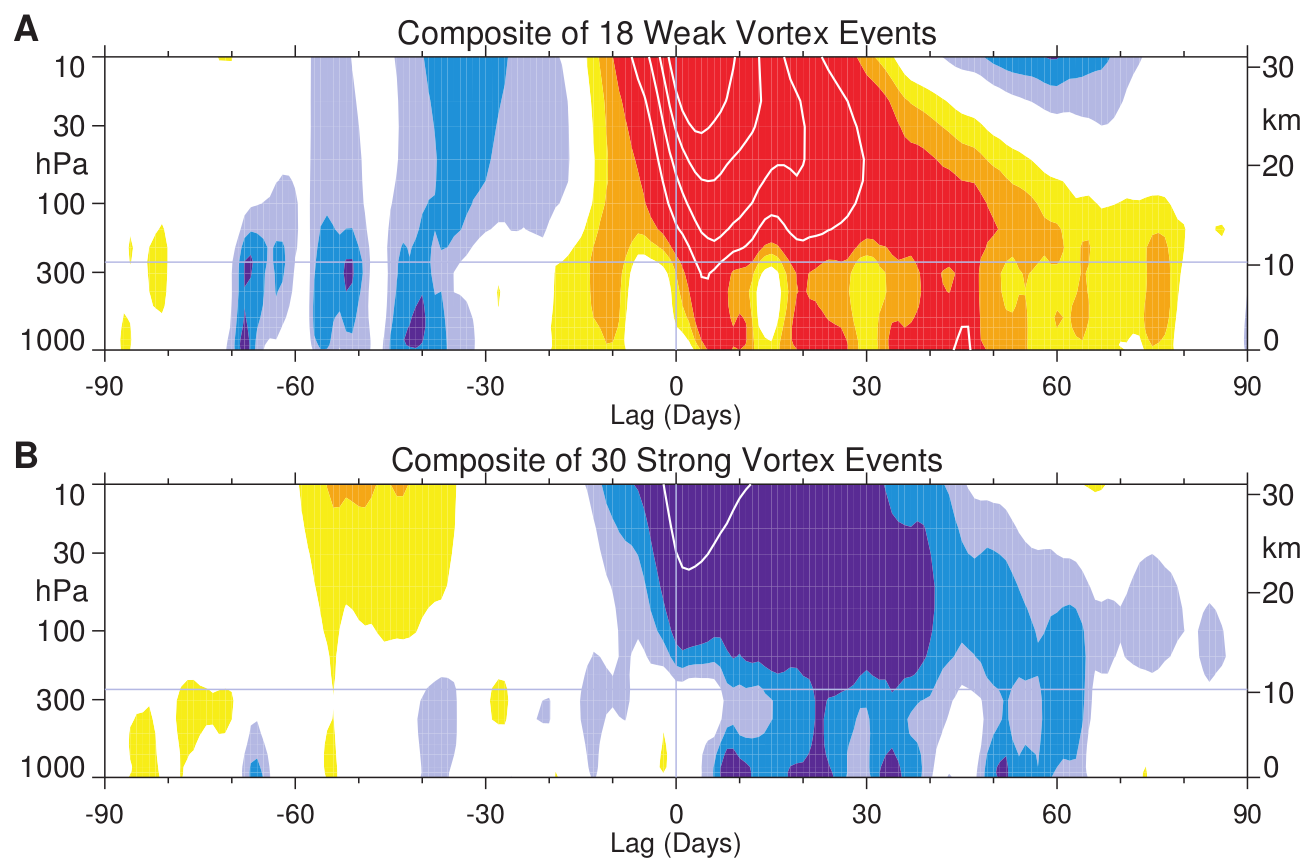
\includegraphics[width=\textwidth]{figures/chapter-intro/Baldwin_Dunkerton.png}
 \caption[NAM composite from \citet{Baldwin2001a}]{Composites of time-height
   development of the northern annular mode for (A) 18 weak vortex events and
   (B) 30 strong vortex events. The events are determined by the dates on which
   the 10-hPa annular mode values cross –3.0 and +1.5, respectively. The indices
   are nondimensional; the contour interval for the color shading is 0.25, and
   0.5 for the white contours. Values between −0.25 and 0.25 are unshaded. The
   thin horizontal lines indicate the approximate boundary between the
   troposphere and the stratosphere. From \citet{Baldwin2001a}.}
 \label{fig:baldwin_dunkerton}
\end{figure}


\subsubsection{Observational evidence}
\label{sec:observ-evid}
\subsubsection{Modelling evidence}
\subsubsection{Mechanisms}
\label{sec:mechanisms}
% Look at Song and Robinson 2004 for basis of mechanisms review


\section{Thesis plan}

\begin{figure}
 \centering
 \noindent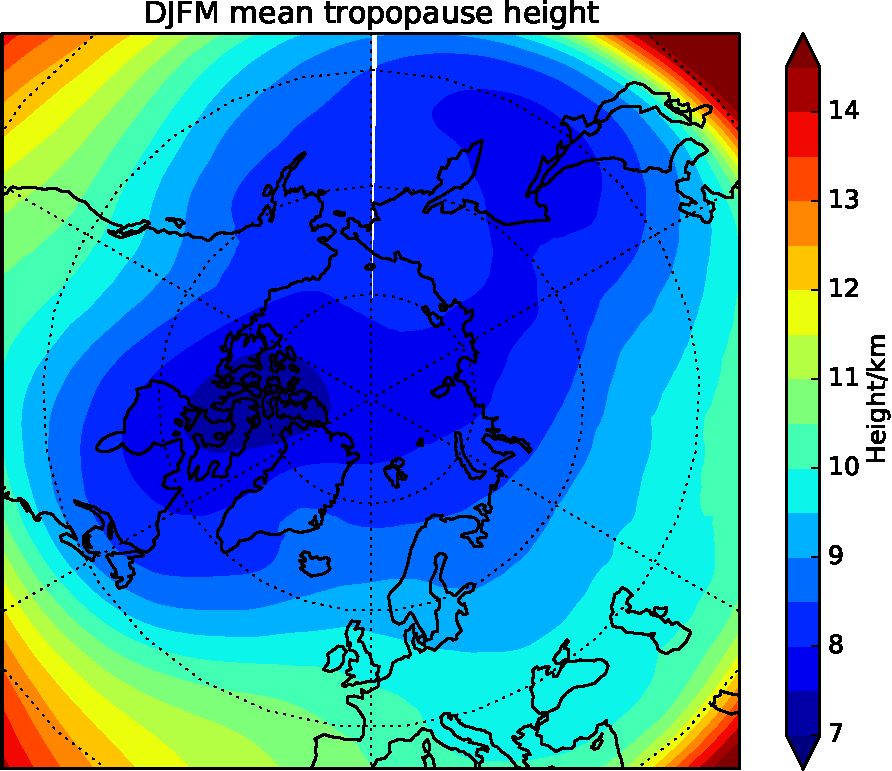
\includegraphics[width=0.5\textwidth]{figures/chapter-intro/mean_tropopause_height.pdf}
 \caption[]{ }
 \label{fig:cmip5_mslp_diff}
\end{figure}



%%% Local Variables:
%%% mode: latex
%%% TeX-master: "thesis"
%%% End:
